\section{Solving Task and Motion Planning Problems}
\begin{figure}[t]
  \centering
    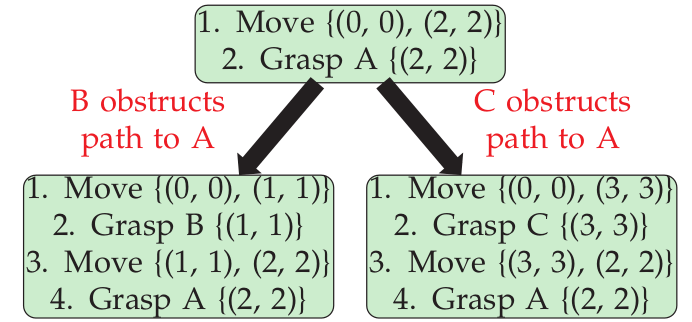
\includegraphics[scale=0.3]{images/ex_prg.png}
  \caption{\small{A simple plan refinement graph for an environment with 3 objects: A,
B, and C. The goal is to grasp object A. Each node maintains a high-level
plan and a set of instantiated continuous values for its symbolic references.
The edges are labeled with errors discovered by the low-level motion planner and
propagated back up to the task planner for replanning.}}
  \label{fig:prg}
\end{figure}

\subsection{SFRCRA-14}
Solving TAMP problems requires evaluation of
possible courses of action comprised of different combinations of
instantiated action operators. This is particularly challenging
because the set of possible action instantiations (and thus the
branching factor of the underlying search problem) is infinite.
We give a brief overview of SFRCRA-14, a recent approach to TAMP, and
refer the interested reader to the cited paper for further details.

SFRCRA-14 solves TAMP problems by: incrementally
searching for a high-level plan that solves the logical abstraction
of the given TAMP problem; determining a prefix of the plan that has a
motion planning feasible refinement; updating the high-level
abstraction to reflect the reason for infeasibility; and searching for
a new plan suffix from the failure step onwards. This search process
addresses the fundamental TAMP problem: high-level
logical descriptions are lossy abstractions of the true environment
dynamics and thus may not include sufficient information to
determine the true applicability of a sequence of actions.

In general, including geometric properties in the logic-based formulation leads to an
increase in the number of objects representing distinct poses and/or trajectories. For
instance, expressing the fact that a trajectory for grasping \emph{can$_1$} is obstructed by
\emph{can$_3$} from the current pose of the robot would require setting a fluent of the
form \emph{obstructs(can$_3$, pose$_{17877}$, trajectory$_{3219}$, can$_1$)} to true in
the description of the high-level state. In turn, this would require adding
\emph{pose$_{17877}$} and \emph{trajectory$_{3219}$} into the set of objects if they were
not already included. Unfortunately, the size of the abstracted, logic-based state space
grows exponentially with the number of objects, and such an approach quickly leads to
unsolvable task planning problems.

SFRCRA-14 addresses this challenge by abstracting the continuous
action arguments, such as robot grasping poses and trajectories, into
a \emph{bounded} set of symbolic references to potential values. A
\emph{high-level}, or \emph{symbolic}, plan refers to the fixed task
sequence returned by a task planner and comprised of these symbolic
references. An \emph{interface layer} conducts plan refinement,
searching for instantiations of continuous values for symbolic
references while ensuring action feasibility.  The resulting process
is able to utilize off-the-shelf task and motion planners while
carrying out the necessary exchange of information in a scalable
manner.

\subsection{Plan Refinement Graph}
Unpublished work recently submitted for review to ICRA 2016 builds on SFRCRA-14 and develops a complete algorithm
that maintains a \emph{plan refinement graph} (PRGraph). Every node $u$ in the PRGraph
represents a high-level plan $\pi_u$ and the current state of the search
for a refinement. An edge $(u,v)$ in the PRGraph
represents a ``correction'' of $\pi_u$ for a specific instantiation of
the symbolic references in $\pi_u$. Let $\pi_{u,k}$ be the plan prefix of
$\pi_u$ consisting of the first $k$ actions. Formally, each edge
$e=(u,v)$ is labeled with a tuple $\langle \sigma, k, \varphi \rangle$.
$\sigma$ denotes an instantiation of references for a prefix $\pi_{u,k}$ of
$\pi_u$ such that feasible motion plans have been found for all
previous actions $\pi_{u,k-1}$. $\varphi$ denotes a conjunctive formula
consisting of fluent literals
that were required in the preconditions of the $k^{th}$ action in
$\pi_u$ but were not true in the state obtained upon
application of $\pi_{u,k-1}$ with the instantiation $\sigma_k$.  The
plan in node $v$ (if any) retains the prefix $\pi_{u,k-1}$ and solves
the new high-level problem which incorporates the discovered facts $\varphi_{u,v}$
in the $k^{th}$ state.

The overall search algorithm then interleaves the search for feasible
refinements of each high-level plan with the addition into the
PRGraph of new edges and plan nodes using the semantics described above.

\figref{fig:prg} illustrates a simple example of a PRGraph.

\subsection{Previous Approach for Learning to Search the PRGraph}
Chitnis et al.~\cite{chitnis2015mlpc} explain that the high level has a two-tiered
decision to make: which node in the PRGraph to
visit next, and whether to 1) attempt to refine this node or 2) quickly generate failure information
from it, thus spawning a child node. They develop heuristics that are trained to estimate
the difficulty associated with refining a plan, in order to make this decision intelligently.

To select among the potential refinement options, the authors train two decision tree regressors
that determine how many iterations would be needed to achieve a valid refinement for a node, or for a child
of that node which incorporates a single additional geometric fact about the environment.
To obtain an estimate for a full plan, they sum this number across all of the plan's actions.
The implicit assumption being made here is that dependencies in plans are, in some way, local:
the plan must be factorizable into subportions with independent refinements.

At test time, they use the regressors to find the best two-tiered action to take at each step.
For example, if refining a child node would reduce the number of steps to a valid refinement,
they bias toward generating a child node.